\documentclass[11pt,final,fleqn]{article}


\usepackage{alltt}

% Basic packages
\usepackage[margin=1in] { geometry }

% Figures
\usepackage[font={bf}]{caption}
\captionsetup{belowskip=10pt,aboveskip=-5pt}
\usepackage{float}
\usepackage[export]{adjustbox}
\renewcommand{\thefigure}{S\arabic{figure}}

% Title
\title{Supplemental Appendix: Penalized regression for left-truncated and right-censored survival data}
\author{Author list}
\date{\today}

\begin{document}
\maketitle

\begin{figure}[h]
\centering
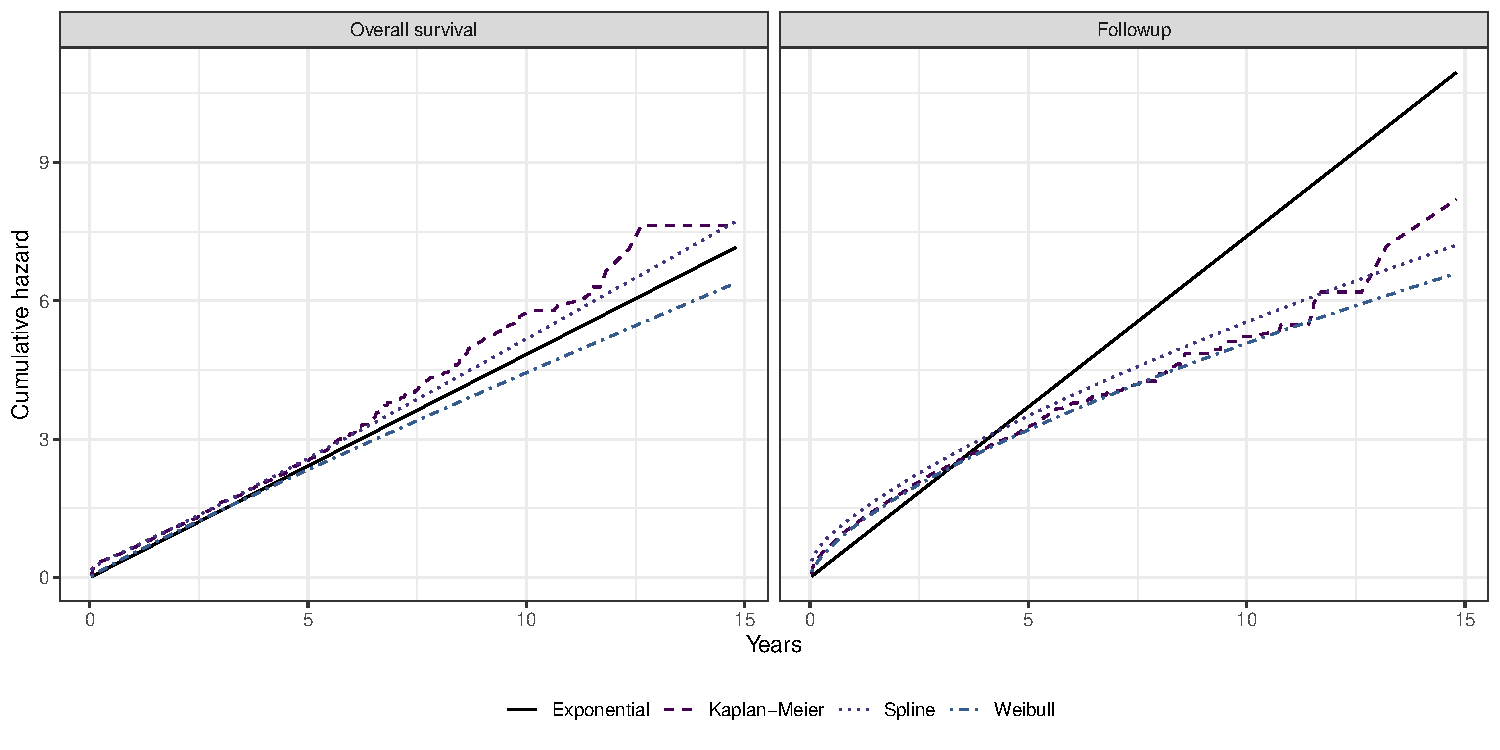
\includegraphics[max size={\textwidth}]{figs/sim_calibration_cumhaz.pdf} 
\caption{Cumulative hazards among non-small cell lung cancer patients in the CGDB in models adjusting for right censoring and left truncation}
\begin{minipage}{\linewidth}
\footnotesize
Notes: The left and right facets plot cumulative hazards for overall survival (i.e., time to death) and followup time (i.e., time to right censoring), respectively. Estimates in the rightmost plot use a ``reverse Kaplan-Meier'' approach whereby the meaning of an event and censoring are flipped. The spline models were fit with one internal knot at the median of the log of followup time. 
\end{minipage}
\end{figure}

\begin{figure}[h]
\centering
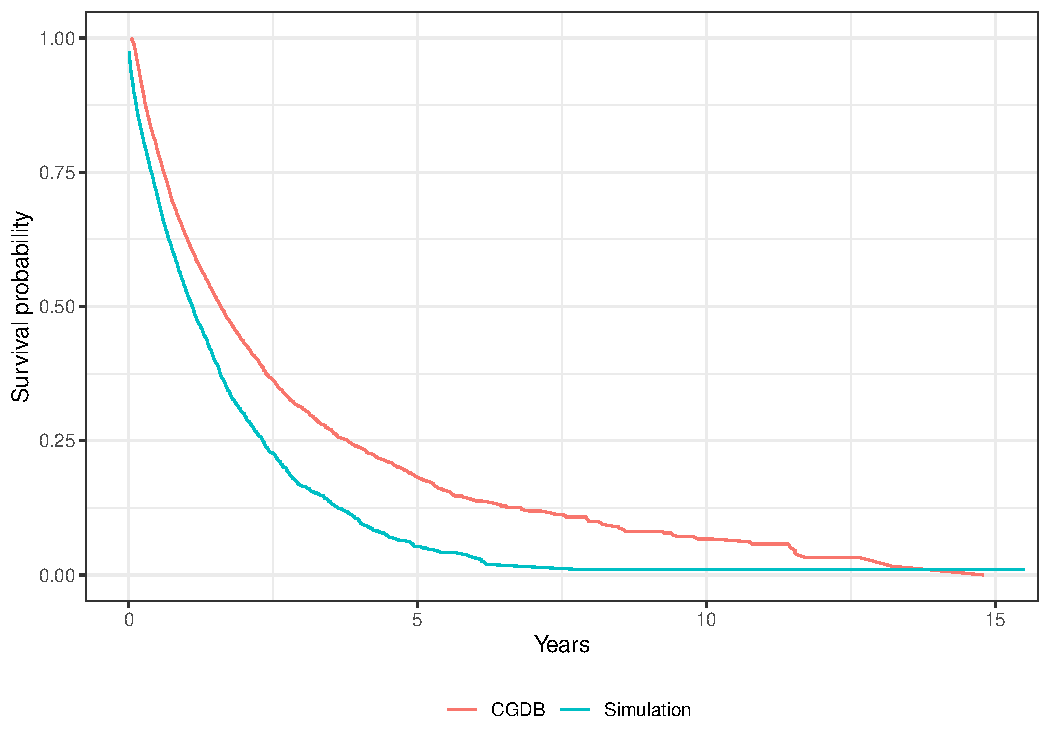
\includegraphics[max size={\textwidth}]{figs/sim_int_km_plot_rwd_v_sim.pdf} 
\caption{Kaplan-Meier plots of overall survival from models that adjust for right censoring but not left truncation in the simulated data and CGDB}
\begin{minipage}{\linewidth}
\footnotesize
Notes: The simulated dataset was simulated using an intercept only Weibull model with no predictors. Only non-truncated patients from the simulation were used for estimation. 
\end{minipage}
\end{figure}



\end{document}